\section{Combinational Logic}
Combinational logic is a type of digital logic in which the output of the logic is a pure function of its present inputs \cite{comblog_wiki}.This means that combinational logic is memoryless; it is not affected by any previous outputs. This is in contrast to sequential logic, for which the output is dependent on present input values and some internal state derived from previous outputs.

\subsection{Boolean Operators and Algebra}
There exist three fundamental Boolean operators:
\begin{itemize}
    \item \textbf{NOT}, a unary operator which outputs the inverse of the input.
    \item \textbf{AND}, a binary operator which outputs HIGH when both inputs are HIGH and LOW otherwise. Denoted by 
    \item \textbf{OR}, a binary operator which outputs HIGH when either of the inputs are HIGH, and LOW otherwise
\end{itemize}

All other Boolean operators, can be derived through a combination of these three fundamental operators. As mentioned in the introduction, one of the ways of representing combinational logic is using Boolean algebra; with the function $Outputs = f(Inputs)$. An example of such a function would be: \\
\begin{center}
Consider $A,B,C$ as inputs, $D$ as output. 
    \begin{equation}
        D = \overline{(A.B + A.C)}
    \end{equation}
\end{center}

One way of simplifying combinational logic is to represent it as a Boolean expression, and simplify it using the rules of Boolean algebra and any other theorems. 

\begin{figure} [h]
    \centering
    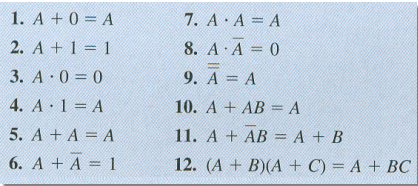
\includegraphics{img/BooleanLaws.png}
    \caption{Rules of Boolean Algebra \cite{boolalg_laws}}
    \label{fig:boolalg_laws}
\end{figure}

Figure \ref{fig:boolalg_laws} shows the rules of Boolean algebra.




\subfloat[Truth Table for the a 2-bit Multiplexer]{
    \begin{tabular}{c|c|c||c}
     \textbf{A} & \textbf{B} & \textbf{S} & \textbf{OUT} \\
     \hline
     0 & 0 & 0 & 0 \\
     0 & 0 & 1 & 0 \\
     0 & 1 & 0 & 0\\
     0 & 1 & 1 & 1\\
     1 & 0 & 0 & 1\\
     1 & 0 & 1 & 0\\
     1 & 1 & 0 & 1\\
     1 & 1 & 1 & 1
    \end{tabular}}